\section{公开继承与受保护成员}
\subsection*{基本语法}
继承的基本语法就是在定义\footnote{虽然在声明类时偶尔也可以这样做,但是我不推荐如此,因为在进行继承时编译器必须已经知道对应基类的定义。}一个类时,用冒号加``继承方式''和``基类名''的形式来表明它按何种方式继承自哪个类。
\begin{lstlisting}
class Base {
    //...
}; //Base类定义已毕
class Derived : public Base { //按public方式继承自Base类
    //...
}; //Derived公开继承自Base
\end{lstlisting}\par
其中的继承方式分为 \lstinline@public@, \lstinline@protected@ 和 \lstinline@private@ 三种,在本节中我们先讲 \lstinline@public@,即公有继承。\par
\subsection*{继承方式与访问权限}
我们已经很熟悉``访问权限''这个概念了。访问权限关乎一个成员是否对外界可见:
\begin{itemize}
    \item \lstinline@public@ 成员对外完全可见。
    \item \lstinline@private@ 成员对外完全不可见。
    \item \lstinline@protected@ 成员比较特殊,我们稍后讲到。这些成员对外界不可见,但对该类的派生类可见。
\end{itemize}
我们说,一个派生类对象具有基类的成员,比如 \lstinline@Husky@ 就有 \lstinline@age@ 和 \lstinline@weight@。那么在派生类中,这些基类的成员又是何种访问权限呢?这是由``基类成员访问权限''和``继承方式''二者共同决定的,见表9.1。\par
\begin{table}[htbp]
\centering
\begin{tabular}{cccccc}
\hline
\rule{0pt}{2.4ex}
\multirow{2}{*}{继承方式} & 基类成员权限 & \multirow{2}{*}{\lstinline@public@} & \multirow{2}{*}{\lstinline@protected@} & \multirow{2}{*}{\lstinline@private@} \\
\cline{2-2}
\rule{0pt}{2.4ex}
& 派生类成员权限 & & & \\
\hline
\hline
\rule{0pt}{2.4ex}
\lstinline@public@ & & \lstinline@public@ & \lstinline@protected@ & 不可见\\
\hline
\rule{0pt}{2.4ex}
\lstinline@protected@ & & \lstinline@protected@ & \lstinline@protected@ & 不可见\\
\hline
\rule{0pt}{2.4ex}
\lstinline@private@ & & \lstinline@private@ & \lstinline@private@ & 不可见\\
\hline
\end{tabular}
\caption{派生类的成员访问权限取决于基类成员访问权限和继承方式}
\end{table}
其中的 \lstinline@protected@ 成员(受保护成员)访问权限对于读者来说是个全新的概念,下面我就来解释一下它的作用和优缺点。\par
\subsection*{\texttt{protected}成员}
我们谈过,\lstinline@private@ 成员的优点在于它是封闭的,只对类内可见。但对于继承来说,它也可能是个麻烦。\par
举个例子,\lstinline@Husky@ 类中的 \lstinline@destory@ 成员函数需要用到 \lstinline@weight@ 这个成员变量。如果我们像上一节中那样在 \lstinline@Dog@ 类中把 \lstinline@weight@ 定义为 \lstinline@public@\footnote{我们此前提过,\lstinline@struct@ 成员的默认访问权限均为 \lstinline@public@;\lstinline@struct@ 类的默认继承方式也是 \lstinline@public@。所以 \lstinline@Dog@ 类中的成员都是公有成员,而 \lstinline@Husky@ 类以公开方式继承 \lstinline@Dog@ 类。},那么无论 \lstinline@Husky@ 类还是其它无关的外界类/函数都有了修改 \lstinline@weight@ 的权限,这是很危险的;然而,如果我们把 \lstinline@weight@ 定义成 \lstinline@private@,那么无论 \lstinline@Husky@ 还是其它外界类/函数都不能访问 \lstinline@weight@\footnote{一种观点认为,\lstinline@private@ 成员是``不可继承''的,换句话说,基类的私有成员并不是派生类的成员。这种看法是合理的,因为一个类的成员总该对这个类可见;如果对这个类都不可见,那么它也算不上是这个类的成员。不过笔者在这里顾及理解上方便,还是选择这样讲。}。\par
而 \lstinline@protected@ 则能很好地解决这个问题。基类的 \lstinline@protected@ 成员对于外界来说是不可见的,但它对于这个类的派生类来说则是可见的,如图9.2所示。\par
\begin{figure}[htbp]
    \centering
    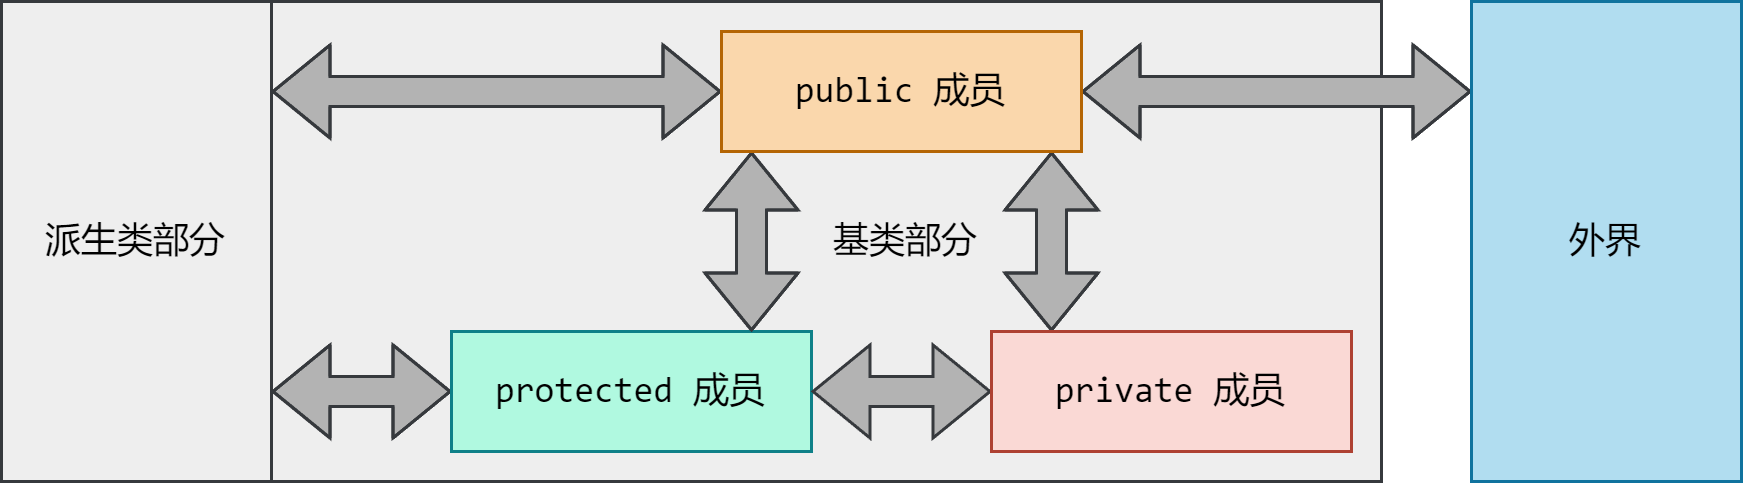
\includegraphics[width=\textwidth]{../images/generalized_parts/09_protected_members_300.png}
    \caption{\lstinline@protected@ 成员对外的可见性}
\end{figure}
有了 \lstinline@protected@ 之后,我们可以这样写:
\begin{lstlisting}
class Dog {
protected: //受保护成员,对外不可见,但对Dog的派生类可见
    unsigned _age; //所有狗都有年龄属性
    double _weight; //所有狗都有体重属性
};
class Husky : public Dog { //公有方式继承自Dog
    //这个类拥有成员age和weight,成员权限为protected
public: //公有成员,对外界可见
    void destroy() { /*...*/ }; //哈士奇独特的拆家本领
};
\end{lstlisting}\par
这样一来,\lstinline@_age@ 和 \lstinline@_weight@ 就对 \lstinline@Husky@ 类可见,使 \lstinline@Husky@ 类的函数可以方便地访问这些成员;同时它们又对无关的其它类不可见,保证了成员不受篡改的安全性。\par
\subsection*{构造与初始化}
派生类拥有它基类的成员,这个关系很像是,一个派生类对象当中内嵌了一个基类对象。
\begin{figure}[htbp]
    \centering
    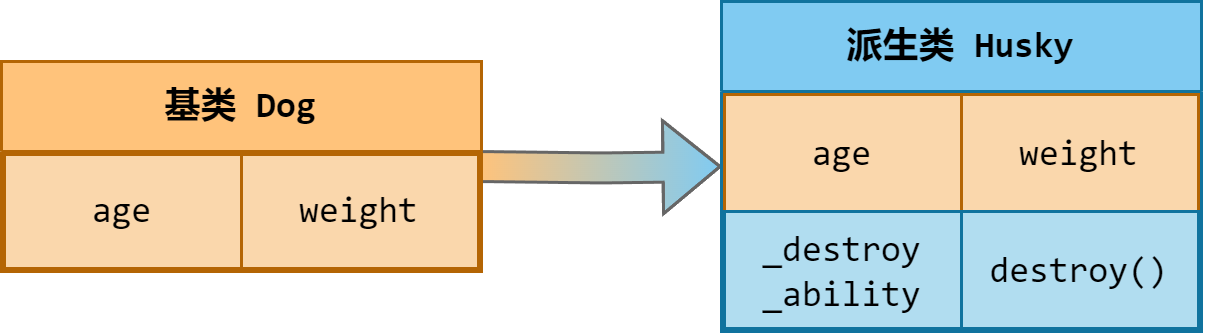
\includegraphics[width=.8\textwidth]{images/generalized_parts/09_built_in_base_class_object_in_derived_class_300.png}
    \caption{一个派生类对象当中内嵌了一个基类对象}
\end{figure}
所以当我们需要对基类对象进行初始化时,也不是按照``成员''进行初始化,而是把基类的对象当作一个整体,调用基类的构造函数进行初始化。\par
\begin{lstlisting}
class Dog {
protected: //受保护成员,对外不可见,但对Dog的派生类可见
    Dog(unsigned age, double weight) : _age {age}, _weight {weight} {}
    //如果把Dog的构造函数定义成protected权限,那么只有其派生类才能正常调用它
    unsigned _age; //所有狗都有年龄属性
    double _weight; //所有狗都有体重属性
};
class Husky : public Dog { //哈士奇类,公有方式继承自Dog
    //这个类拥有成员age和weight,成员权限为protected
private:
    int _destroy_ability; //拆家能力
public:
    Husky(unsigned age, double weight, int ability)
        : Dog {age, weight}, _destroy_ability {ability}
    {} //初始化内嵌Dog对象的成员,以及_destroy_ability成员
    void destroy() { /*...*/ }; //哈士奇独特的拆家本领
};
class Retriever : public Dog { //金毛寻回犬类,公有方式继承自Dog
    //这个类拥有成员age和weight,成员权限为protected
private:
    int _guide_ability; //导盲能力
public:
    Retriever(unsigned age, double weight, int ability)
        : Dog {age, weight}, _guide_ability {ability}
    {} //初始化内嵌Dog对象的成员,以及_guide_ability成员
    void guide() { /*...*/ } //金毛独特的导盲本领
};
\end{lstlisting}\par
在这里,我们把 \lstinline@Dog@ 类的构造函数定义成受保护成员。按前文所述,这些成员对派生类以外的外界都是不可见的,所以我们不能在外部使用这个函数来进行构造\footnote{其实这个类还有一个作为公有成员的默认拷贝构造函数,所以确实还存在这样的方法使我们能够在外部定义对象。}。换言之,我们这样就保证了:在外界中不能直接定义 \lstinline@Dog@ 类对象,只能定义它的派生类的对象\footnote{不过,从另一个意义上讲,派生类的对象也是基类的对象。}。\par
两个派生类 \lstinline@Husky@ 和 \lstinline@Retriever@ 对象的构造函数都是公有的,我们就可以在类外调用了。它们都接收三个参数,分别是 \lstinline@age@, \lstinline@weight@, \lstinline@ability@。所以我们可以这样定义对象:
\begin{lstlisting}
int main() {
    Husky mine {5, 27, 1000000};
    Retriever zhang3 {4, 25.67, 99};
}
\end{lstlisting}
在创建 \lstinline@mine@ 对象时,程序将调用 \lstinline@Husky::Husky(unsigned,double,int)@ 函数,那么这个函数做了什么呢?
\begin{lstlisting}
public:
    Husky(unsigned age, double weight, int ability)
        : Dog {age, weight}, _destroy_ability {ability}
    {}
\end{lstlisting}\par
我们看到,这个函数在初始化时,其 \lstinline@Dog@ 成员部分是通过调用 \lstinline@Dog@ 类的构造函数来集中解决的;而独属于 \lstinline@Husky@ 的那部分,才是单独处理的。这一点对三种继承方式来说都是通用的——来自基类的成员,需要通过基类的构造函数来进行初始化。即便我们在代码中没有这么写,基类的构造函数也是会被调用的。我们可以用这段代码来验证之:
\begin{lstlisting}
struct Base { //struct成员默认为public成员,这里图方便就用struct了
    Base() { //Base的默认构造函数
        std::cout << "Base::Base() is called." << std::endl;
    }
};
struct Derived : Base { //struct类的默认继承方式也是公开继承
    Derived() { //在Derived构造函数当中并没有写明要调用Base的构造函数
        std::cout << "Derived::Derived() is called." << std::endl;
    }
};
int main() {
    Derived de; //定义Derived类的对象,预期会调用Derived类的构造函数
}
\end{lstlisting}
这段代码的运行结果如下:\\\noindent\rule{\linewidth}{.2pt}\texttt{
Base::Base() is called.\\
Derived::Derived() is called.
}\\\noindent\rule{\linewidth}{.2pt}
这段代码能体现出两条信息:其一,在调用派生类的构造函数时,基类的构造函数也会被自动调用;其二,基类构造函数体的执行要早于派生类的构造函数体\footnote{注意,这是函数体的执行顺序!这个实验并没有验证初值列的顺序。}。\par
\subsection*{析构}
不只是构造函数,派生类的析构函数在调用时,也会调用基类的析构函数。我们同样根据一个例子来看它的效果。
\begin{lstlisting}
struct Base {
    ~Base() { //Base的析构函数
        std::cout << "Base::~Base() is called." << std::endl;
    }
};
struct Derived : Base {
    ~Derived() { //Derived的析构函数
        std::cout << "Derived::~Derived() is called." << std::endl;
    }
};
int main() {
    Derived de;
}
\end{lstlisting}
这段代码的运行结果如下:\\\noindent\rule{\linewidth}{.2pt}\texttt{
Derived::~Derived() is called.\\
Base::~Base() is called.
}\\\noindent\rule{\linewidth}{.2pt}
我们发现,对象销毁时析构函数的调用顺序,与对象创建时构造函数的调用顺序,刚好是相反的。在析构的时候,派生类的析构函数先调用,然后才是基类的析构函数。\par
也正因为,派生类的析构函数总是要调用基类的析构函数,所以我们根本不需要在写派生类时还要为了``基类成员的内存泄漏''而提心吊胆(只要你写的基类没有这个问题)。
\begin{lstlisting}
class stack : std::vector<int> { //class的默认继承方式为private
public:
    //...
    ~stack() {} //无需为std::vector<int>的动态内存而担扰!自有它的析构函数来回收
};
\end{lstlisting}\par
